\chapter{The Observer}

\vspace{1em}
\hfill
\begin{minipage}[c]{0.55\textwidth}
\raggedleft
\small\itshape
Every quantum transition taking place on every star, in every galaxy, in every remote corner of the universe, is splitting our local world into myriads of copies of itself.\\[0.5em]
\upshape\footnotesize Bryce DeWitt, ``Quantum Mechanics and Reality'' (1970)
\end{minipage}%
\hspace{0.5em}
\begin{minipage}[c]{0.12\textwidth}
% \includegraphics[width=\textwidth]{figures/ch08_observer.png}
\end{minipage}
\vspace{1.5em}

\noindent Chapter 7 ended with a promise. \emph{Two routes to the same Library.} This chapter takes the second.

The first route was the slip: read the universal prior ontologically (CUH) and the Library becomes populated with realities. The second route does not require CUH. It comes from quantum mechanics, on a particular reading of what the equations are about.

\section*{Move III: Many-Worlds}

Quantum mechanics has had an interpretation problem since the 1920s. The mathematics works exquisitely. Predictions match experiments to extraordinary precision, in some cases to one part in $10^{12}$. The question is what the mathematics is \emph{about}.

The orthodox view, Copenhagen, says: the wave function describes what the observer knows; measurement is a special process that ``collapses'' the wave function to a definite outcome. This is operationally fine but structurally awkward. Why is measurement special? What counts as a measurement? Where is the boundary between the observed system and the observer?

In 1957, Hugh Everett proposed a different reading. The wave function is the complete description of physical reality. There is no collapse. When you measure a quantum system, the wave function of you-plus-system continues to evolve unitarily, splitting into branches: one branch in which you observed outcome $A$, another in which you observed outcome $B$. Both branches are equally real. The branches do not interact at macroscopic scales, because decoherence rapidly suppresses any interference between configurations that differ in many degrees of freedom.\footnote{Decoherence is established mathematics, independent of MWI. It explains why definite outcomes are observed without requiring a collapse postulate. MWI takes the decoherent branch structure as ontologically real; Copenhagen treats it operationally.} From inside any one branch, the result of the measurement looks definite. From outside, every result happened.

This is the Many-Worlds Interpretation. It is the chapter's third labeled move.

\textbf{Move III: Many-Worlds.} The wave function is the complete description of physical reality. There is no collapse. Branching is real. Each branch contains observers experiencing definite outcomes.

\begin{figure}[h]
\centering
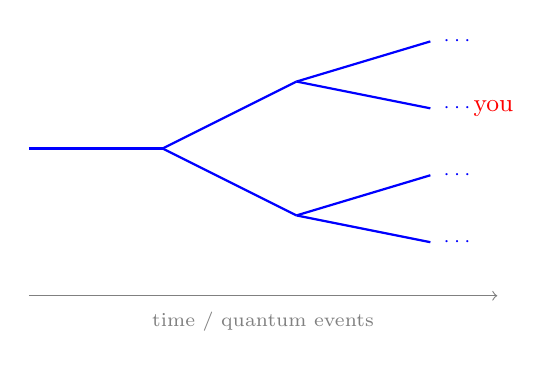
\begin{tikzpicture}[scale=0.85]
  % Trunk
  \draw[thick, blue] (0, 1) -- (2, 1);

  % First branch at t1
  \draw[thick, blue] (2, 1) -- (4, 2);
  \draw[thick, blue] (2, 1) -- (4, 0);

  % Second branches at t2
  \draw[thick, blue] (4, 2) -- (6, 2.6);
  \draw[thick, blue] (4, 2) -- (6, 1.6);
  \draw[thick, blue] (4, 0) -- (6, 0.6);
  \draw[thick, blue] (4, 0) -- (6, -0.4);

  % Continuation
  \node[font=\scriptsize, blue] at (6.4, 2.6) {$\cdots$};
  \node[font=\scriptsize, blue] at (6.4, 1.6) {$\cdots$};
  \node[font=\scriptsize, blue] at (6.4, 0.6) {$\cdots$};
  \node[font=\scriptsize, blue] at (6.4, -0.4) {$\cdots$};

  % Time axis
  \draw[->, gray] (0, -1.2) -- (7, -1.2);
  \node[font=\scriptsize, gray, anchor=north] at (3.5, -1.3) {time / quantum events};

  % "You" annotation on one branch
  \node[font=\small, red, anchor=west] at (6.5, 1.6) {you};
\end{tikzpicture}
\caption{MWI branching. At each quantum event, the wave function splits into decoherent branches corresponding to each possible outcome. Branches do not interfere at macroscopic scales. Each branch contains a version of every observer present at the event. ``You'' are in one branch; copies of ``you'' inhabit the others.}
\label{fig:mwi-branching}
\end{figure}

What it buys. A second, independent route to the multiverse. The same conclusion (you exist in many branches) is reached without invoking CUH or any algorithmic ontology. Quantum mechanics, taken at face value, gives multiplicity for free.

What it costs. A specific interpretation of QM. Other interpretations (Copenhagen, Bohmian mechanics, spontaneous-collapse theories like GRW) avoid the branching but pay their own costs. MWI is the cleanest reading of the unmodified equations, but it is not forced. The Born rule (why outcomes have probabilities proportional to $|\psi|^2$ rather than uniform measure on branches) is a standing puzzle that MWI must address, and the literature on it is large.

\section*{The Library inside our physics}

A clarification on the apparent symmetry between Move II and Move III. Both arrive at a multiverse, but they are not equivalent in cost.

CUH (Move II) is a philosophical commitment. It asks the reader to accept that all computable structures exist as actual realities. This is a substantial metaphysical addition to ordinary realism. It is defensible (the cut argument of Chapter 6 makes the case) but it is a real cost.

MWI (Move III) is a reading of equations we have already accepted. Quantum mechanics is the most experimentally confirmed theory in the history of science, accurate in some predictions to one part in $10^{12}$. The wave function and its unitary evolution are the standard description. MWI asks only that no collapse postulate be added: take the equations at face value, let the wave function evolve as it does, accept that decoherent branches are real. The reader who refuses MWI must adopt some other interpretation that adds something: a collapse mechanism (Copenhagen), hidden variables (Bohmian mechanics), spontaneous-collapse dynamics (GRW). Each adds a postulate that the unmodified theory does not require. The burden of evidence is on the refuser.

This asymmetry has a consequence. CUH posits a Library of all computable structures as a separate metaphysical thesis. MWI does not posit a library; it observes one. The wave function of the universe, under the standard unmodified reading, \emph{is} a library-like structure. Every possible outcome of every quantum event exists in some decoherent branch, at its coordinates, with the same ontological status as the outcome you happen to observe. The Library that Chapter 2 introduced as a Borges thought experiment, and that Chapter 6 made into an ontology of computable structures, is, under MWI, already in our physics. It was not posited. It is in the equations.

This makes MWI by itself a route to almost everything that comes next. The Library inside our physics is enough to permit Boltzmann-like fluctuations (given enough cosmic time), branches in which suffering is maximized for indefinite stretches, branches in which any physically realizable history of any observer has played out. CUH adds further structure (the full ontology of computable structures, not just our universe's branches) but is not required for most of the cascade. A reader who refuses CUH but accepts MWI still inherits most of the framework's costs.

Convergent evidence remains. CUH and MWI come from different traditions and arrive at the same picture. But the cleaner statement is this: MWI gives a library of branches inside our physics; CUH puts a larger library on top, philosophically. The convergence is between physics and philosophy meeting in the same place.

\section*{What an observer is}

The chapter has used the word \emph{observer} without saying what one is. The framework needs a working definition before the next question makes sense.

An observer is a substructure of the wave function (under MWI) or of $U(p)$ (under CUH): a local region with internal organization, a sensorium, a memory, a capacity to model. Nothing in the framework makes observers different in kind from any other substructure. They are computable patterns, like everything else.

But not every substructure is an observer. Observers need something specific from the universe they are in.

\emph{Hierarchical decomposability.} An observer's predictions, models, and actions all rely on isolating subsystems. The cell can be modeled without the quarks. The apple's fall can be predicted without the wave function of every electron. For this to work at all, the universe (whether $U(p)$ or the relevant branch of the wave function) must have a hierarchical structure: at each scale, local short programs approximate local substructures well enough for the observer to reason. Without this, no observer could form a coherent model of anything.

This is a strong restriction on which programs support observers. The multiverse contains every program. The vast majority do not have local decomposability. Their $U(p)$ is locally chaotic, globally entangled, or perfectly homogeneous with no local features. None of these admit observers doing science.

We exist in programs whose $U(p)$ is locally decomposable at multiple scales. This is anthropic: we observe what supports observation. But it is more substantive than the usual anthropic move. It is not just that we are in a universe with us in it. It is that the universe has compositional structure across scales, and the existence of effective theories at every scale we have probed is direct evidence of this.

\emph{Local inference.} The observer's epistemic activity, science, is not a search for the global program. The shortest program that produces the full universe is uncomputable to find, and an observer with finite resources could never carry out the search even as approximation. What the observer does instead is build a collection of short local programs $p_s$, each approximating a local substructure $s$. These are the effective theories of physics, the laws of biology, the heuristics of everyday cognition. Together they form the observer's working model of its local region.

The observer never has access to the global program. The observer has access to a prefix of its local substructure, restricted to whatever its sensorium can resolve. From this, it infers local $p_s$'s and predicts forward. The relevant ensemble is not a posterior over global programs; it is the collection of local effective theories the observer maintains.

This is what science is, in this framework. Not the discovery of \emph{the} program. The construction of a library of local approximations, scale by scale, each anchored to a substructure the observer can probe.

\emph{The self as a local model.} The same picture extends to the observer's self-representation. The brain's model of itself is a short local program approximating the substructure the observer occupies. $I$ is one of the local theories. The dissolution of the self in Chapter 13 follows from this: the self-model is not different in kind from the other local effective theories the observer maintains. The self is a $p_{\text{self}}$, useful, finite, approximate, and like every other $p_s$, not the structure it describes.

With these in place, the question of the next section sharpens. The observer is a local substructure of the multiverse, doing local inference, with no access to global structure. So: which substructure is the observer? Which version, in which branch, is \emph{you}?

\section*{Where am I?}

With many realities (or many branches) on the table, a sharp question emerges. Among all the observers in the multiverse who match your current self-description (your memories, your sensory state, your moment of reading this), which one is you?

The literature has attempted to answer this with specific indexical assumptions. The \emph{Self-Sampling Assumption} (SSA) says reason as if you are a random sample from some reference class of observers. The \emph{Self-Indication Assumption} (SIA) says your existence is evidence for universes with many observers. These assumptions disagree about the Sleeping Beauty problem, the doomsday argument, and the Boltzmann brain problem. Neither is forced. Both are defensible. Both have known difficulties.

The book does not commit to any specific indexical assumption. The question \emph{where am I?} is one of the questions the framework permits us to pose but does not give a unique answer to. This is not a hole in the bedrock. It is an honest acknowledgment that not every question the framework lets us ask has a sharp formal answer.

\section*{What the framework permits}

The framework, with Moves I, II, and III taken, permits a great deal that is uncomfortable to sit with. Most of what follows is already permitted by Move III alone: the Library inside our physics is enough. CUH (Move II) makes the picture larger but is not required to inherit the costs. A small sample.

\emph{Boltzmann brains.} Under naive observer-counting in a long-lived universe, you might be a momentary thermodynamic fluctuation with no real past. Your memories of yesterday refer to nothing; you will dissolve in seconds. The book does not refute this. Various technical responses exist; none is fully satisfying.\footnote{Schmidhuber's \emph{speed prior} is one computable approximation to $M$ that incidentally suppresses Boltzmann brains by penalizing runtime. It has costs of its own: it disfavors computationally deep structures, including the kind any non-trivial universe presumably is. See Bennett (1988) on logical depth. The book does not adopt the speed prior as a resolution.}

\begin{figure}[h]
\centering
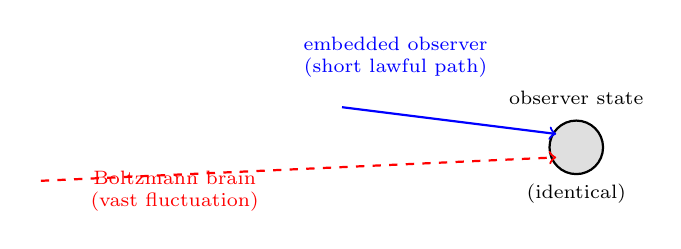
\begin{tikzpicture}[scale=0.85]
  % Common observer state on the right
  \draw[thick, fill=gray!25] (8, 0.8) circle (0.4);
  \node[font=\scriptsize, anchor=south] at (8, 1.3) {observer state};
  \node[font=\scriptsize, anchor=north] at (8, 0.4) {(identical)};

  % Embedded path: short blue arrow from the left
  \draw[thick, blue, ->] (4.5, 1.4) -- (7.7, 1.0);
  \node[font=\scriptsize, anchor=south, blue, text width=3.2cm, align=center] at (5.3, 1.7) {embedded observer (short lawful path)};

  % BB path: very long red dashed arrow from far left
  \draw[thick, red, dashed, ->] (0, 0.3) -- (7.7, 0.65);
  \node[font=\scriptsize, anchor=south, red, text width=3.5cm, align=center] at (2, -0.3) {Boltzmann brain (vast fluctuation)};
\end{tikzpicture}
\caption{Two paths to the same observer-state. An embedded observer (blue) reaches the state through lawful, comparatively rapid processes. A Boltzmann brain (red) reaches the same state through a vast thermodynamic fluctuation. From inside the moment, the two are indistinguishable. The framework does not tell us which we are.}
\label{fig:boltzmann-brain}
\end{figure}

\emph{Hellscapes.} Universes whose laws produce maximal suffering for indeterminate stretches. They exist at their coordinates in the Library. The cut principle of Chapter 6 forbids us from selectively excluding them on simplicity grounds. The measure has no opinion about whether to dislike them.

\emph{Dark quantum continuation.} Under MWI plus an indexical assumption that the first-person sequence follows surviving branches, your subjective experience may continue indefinitely into branches of progressive decay. Death may not arrive in the first person, but what does arrive may be worse than death.

\emph{Versions of you, and of everyone you love, doing or suffering anything specifiable.} For every act of cruelty that is computable, there is a coordinate where some version of you committed it. For every form of suffering that is computable, there is a coordinate where someone you would recognize endures it. The cut principle does not exclude these from existence.

The framework does not resolve any of this. The book does not pretend that it does. These are the costs of taking Moves I, II, III seriously.

What the book offers in response is not a formal move. It is the chosen response of Part II. The mathematics is silent on what to do; care is what we provide; the rest of the book is what that looks like.\footnote{Camus, considering the absurd condition of finite beings in an indifferent cosmos, concluded: \emph{Il faut imaginer Sisyphe heureux}. One must imagine Sisyphus happy. The book's posture is parallel. The framework is what it is. The response is what we choose, in awareness of what the framework permits.}

\section*{What if you refuse}

The book takes Move III. The reader does not have to.

Refuse Move III, and the multiverse from MWI evaporates. You have only the multiplicity from CUH (if you took Move II) or no multiplicity at all (if you also refused Move II). Other interpretations of QM (Copenhagen, Bohmian mechanics, GRW-style spontaneous collapse) avoid the branching but pay their own costs.

The bedrock survives any refusal. Each move adds reach. Each move costs something. The reader can trace any conclusion to the moves it requires.

\section*{Where this leaves you}

Part I closes here. The reader has met three labeled moves:

\begin{itemize}
\item \textbf{Move I:} Church-Turing applied to reality. The world is computable.
\item \textbf{Move II:} Computable Universe Hypothesis. All computable structures exist.
\item \textbf{Move III:} Many-Worlds. The wave function does not collapse; branches are real.
\end{itemize}

The bedrock is closed mathematics. The moves are interpretive commitments. Together they give a multiplicity of realities with the uncomfortable implications the previous section catalogued.

The book does not engineer answers to questions the framework permits but does not resolve. The \emph{where am I?} question stays open. The Boltzmann brain hypothesis stays open. The presence of hellscapes and worse stays in the picture. None of this can be argued away.

What follows is not an argument away. It is the chosen response.

The next chapter states the book's title. Part II is the response.
